\documentclass{article}
\usepackage{projstyle}
\usepackage{graphicx}
\usepackage{mathtools}
\usepackage{enumitem}

\title{A Brief Introduction to Legendrian Knots}
\author{Shreyas Casturi\\Ana Fishburn}
\date{5 November 2018}

\begin{document}

\maketitle

\begin{abstract}
    We will introduce the concept of a Legendrian knot and then discuss
    the various attributes that Legendrian knots have. %specifically
    % as it relates to their dual projections, and more.
    We will also discuss
    a specific class of knot invariants - the classical invariants - for
    Legendrian knots and show how these may be calculated.
% We start by defining Legendrian knots and isotopies of Legendrian knots.
% Then we study the classical invariants of Legendrian knots:
% the topological knot type, the Thurston-Bennequin number, and the rotation number.
% We then explain how, while sufficient for certain classes of knots in tight
% contact structures, there are nonisotopic Legendrian knots with equal
% In particular, we introduce the Chekanov-Eliashberg DGA, and see that its
% homology, the knot contact homology, is an invariant. We see how this
% can be computed to distinguish versions of the $5_2$ knot with equal classical
% invariants.
\end{abstract}

\section{Introduction}
A {\it contact structure} on $\R^3$ is a method of placing a plane at every point,
such that these planes satisfy certain technical conditions.
There are various distinct contact structures we could use, some of them giving
very different properties.
However, for this paper, we will exclusively consider the standard contact structure:
At every point in $\R^3$, we consider the plane spanned by
\[\left\{\frac{\partial}{\partial y},\frac{\partial}{\partial x} + y\frac{\partial}{\partial z}\right\}.\]
Visually, we can see that these planes are always tangent to the $y$-axis, but also
twist around once when moving from $y = -\infty$ to $y = \infty$.

Now that we have this contact structure, we can define a {\it Legendrian knot}
as a knot that is at every point tangent to the plane at that point.
In particular, if we look at the tangent vector $v$ to $K$ at a point $p = (x,y,z)$,
then
\[ v = A\frac{\partial}{\partial y} + B\left(\frac{\partial}{\partial x} +y\frac{\partial}{\partial z}\right)\]
for some real numbers $A$ and $B$.
We can equivalently formulate this condition using a parametrization of $K$ as
the image of a smooth embedding $\phi : [0,1] \to \R^3$, where $\phi(t) = (x(t),y(t),z(t))$ satisfies
\[ z'(t)-y(t)x'(t) = 0.\]

We can now say that two Legendrian knots are equivalent if they can be related by a continuous
family of Legendrian knots. This is very similar to the definition of equivalence
for smooth knots, only here, we restrict the allowable motions.
Therefore, Legendrian equivalence is a finer relation than smooth knot equivalence,
and, in fact, we will show that there are many Legendrian inequivalent knots
with the same smooth knot type.

\section{Projections}
Before we can discuss invariants of Legendrian knots, we must first understand
the ways to visually represent them.
Because Legendrian knots rely on our choice of contact structure, and therefore
our choice of coordinates, dealing with projections of Legendrian knots will
be more complicated than with smooth knots.

The first method of projecting Legendrian knots is the {\it front projection}.
This is the projection onto the $xz$-plane. From the differential equation
$z'(t) = y(t)x'(t)$, we see that we can recover the $y$ coordinate from the front
projection by
\[y(t) = \lim_{t_0\to t}\frac{z'(t)}{x'(t)}.\]
We find the following two properties of front projections:
\begin{enumerate}[label=\roman*)]
\item There may be no vertical tangencies: if $x'(t)$ vanishes, so does $z'(t)$. Instead we 
allow {\it cusps}, points where the diagram forms a sharp horizontal point.
\item At each crossing, the under strand has greater slope than the over strand.
\end{enumerate}
It turns out that these conditions completely characterize front projections:
if $(x(t),z(t))$ satisfies these conditions, they are the coordinates of a Legendrian knot.
Furthermore, for any Legendrian knot, we can arrange for the set of cusp points to be finite.

We can take a projection of a smooth knot and convert it into the front
projection of a Legendrian knot by rotating each crossing until the under
strand has greater slope, and then
replacing vertical tangencies with cusps. We have therefore proved
\begin{theorem}
Every smooth knot may be realized as a Legendrian knot.
\end{theorem}

We now consider the harder to work with, but just as essential, {\it Lagrangian projection}.
This is the projection onto the $xy$-plane. This time, we must recover the $z$ coordinate
by integrating, so up to a constant $z_0$, we have
\[ z(t) = z_0 + \int_0^t y(s)x'(s)\,ds.\]
Now $(x(t),y(t))$ will provide a valid $z(t)$ if and only if
\begin{enumerate}[label=\roman*)]
\item $\int_0^1 y(s)x'(s)\,ds = 0$.
\item $\int_{t_1}^{t_2} y(s)x'(s)\,ds \neq 0$ whenever $(x(t_1),y(t_1))=(x(t_2),y(t_2))$.
\end{enumerate}

\section{Classical Invariants}
We now discuss the classical invariants related to Legendrian knots.

There are three major invariants we will discuss:
\begin{itemize}
    \item \textit{The topological knot type}
    \item \textit{The Thurston-Bennequin number}
    \item \textit{The rotation number}
\end{itemize}

\subsection{The Topological Knot Type}
We consider two \textit{Legendrian knots} as equivalent
if there is a a continuous family of \textit{Legendrian knots} between
them. This is analogous to smooth knot equivalence, though in our case,
the motions/moves allowed to turn one knot into another are restricted,
due to the presence of the contact structure framework.

With this idea in mind, we develop a theorem:
\begin{theorem}
    If two Legendrian knots are Legendrian equivalent, then they are
    equivalent as smooth knots.
\end{theorem}

That is, we may consider their projections not as Lagrangian or front
projections, but simply as projections of a smooth knot. If the \textit{Legendrian knots}
are equivalent, then we can show that they are equivalent as smooth knots.

Therefore, if there is an 
isotopy between two Legendrian knots is, then there is an isotopy of the underlying knot
projections as smooth knots.

This leads to the first major invariant: \textit{the topological knot type}.

For a given \textit{Legendrian knot} L, this invariant is denoted as $k(L)$.
This invariant is the equivalence class of all knots that are smoothly equivalent
to \textit{L}.

We may have various invariants for these
knots be the same, but the underlying types - \textit{figure-eight} and \textit{unknot}
are not the same, and so these two knots cannot be equivalent based on a consideration
of their \textit{topological knot type}. One can convince themselves that
the equivalence class of all knots smoothly equivalent to a \textit{figure-eight}
cannot have the \textit{unknot} in that class.

Let us demonstrate this with a small example.

Let us take a look at a simple example - the \textit{Legendrian unknot} and
\textit{Legendrian figure-eight}. Let us
look at their front diagrams:
\begin{figure}[h!]
    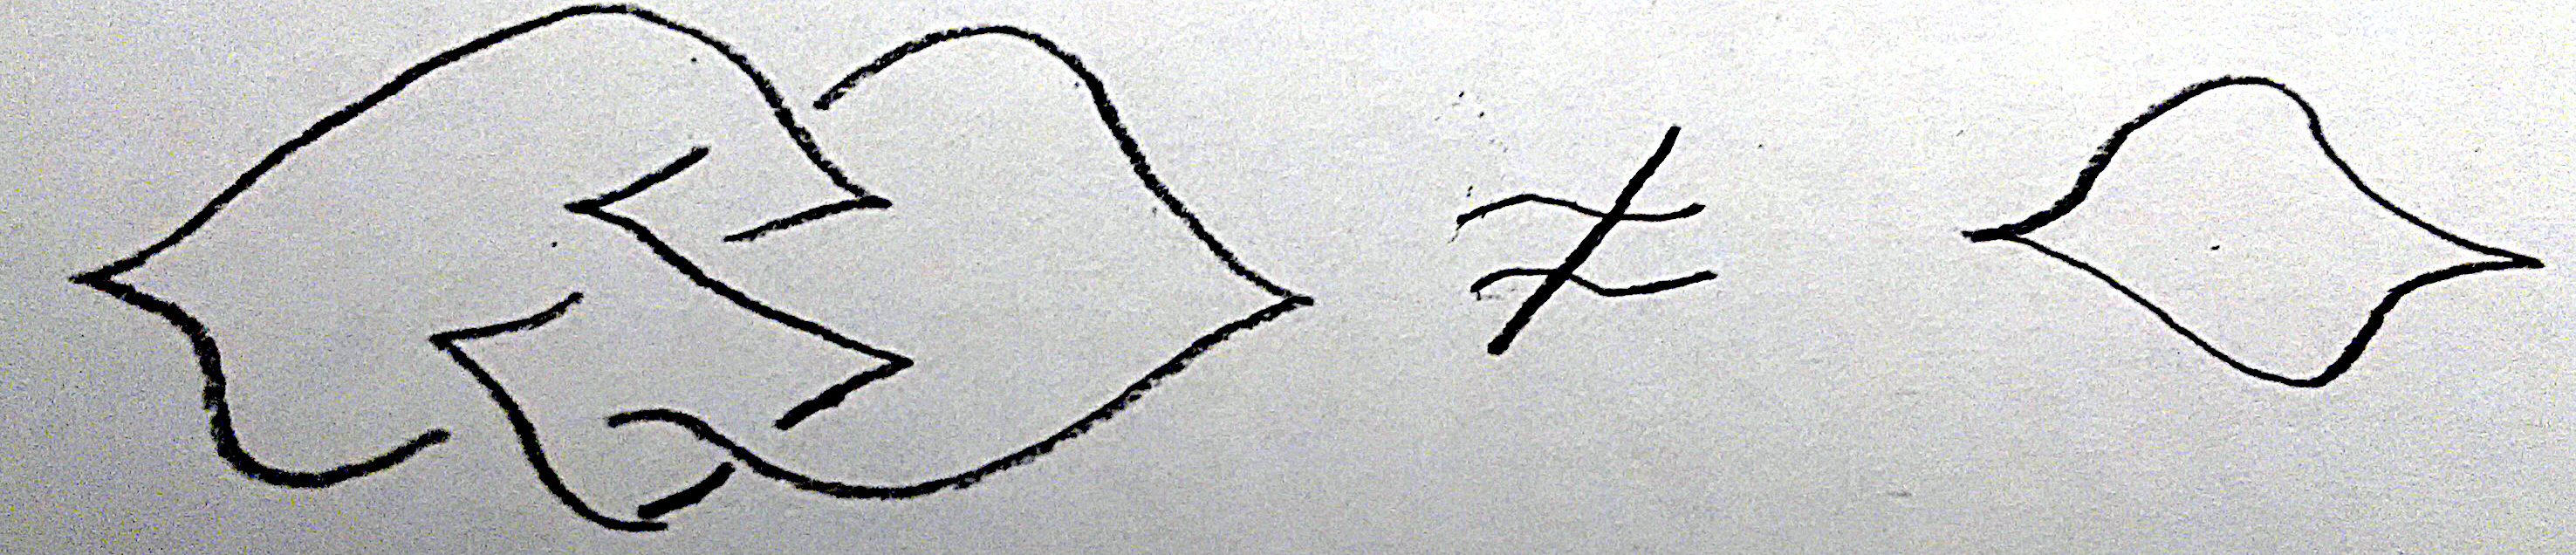
\includegraphics[width=\linewidth]{notEq.jpg}
    \caption{Front projections of non-equivalent Legendrian knots.}
    \label{fig:knot1}
\end{figure}

We note that as the smooth knot types of these projections are not the same,
neither can their \textit{Legendrian knots} be equivalent.

In short, \textit{the topological knot type} is an invariant that uses the smooth
knot type of \textit{Legendrian knot projections} to determine equivalence. If we
know these types aren't the same, then we can assume that the \textit{Legendrian knots}
cannot be the same.

\subsection{Thurston-Bennequin Invariant}

One way in which we can determine if two \textit{Legendrian knots} are equal
is by measuring how much their contact planes "coil" around their knots. However,
we need a way to actually calculate this degree of coiling. This degree of coiling
is called the \textit{Thurston-Bennequin number}, or \textit{invariant}.

Without reverting to a rather geometric definition of this degree, we'll
calculate this degree of coiling by taking a look at the twin projections
\textit{Legendrian knots} have.

\textit{Legendrian knots} have what are called \textit{cusps}. Cusps are points
where the derivative at that point cannot be calculated. That is, the graph/curve
is not differentiable at that point.

One of the stipulations for a knot to be a \textit{Legendrian knot} is
that there can be no vertical tangencies. That is, the knot projection cannot
be differentiable such that the tangent line at a given point is completely
vertical. In order for this to happen, there must be cusps at such points, so that
there can be no vertical tangent lines at these points.

We have one quality of these knot projections called the \textit{right cusp number},
the count of how many cusps there are in a given \textit{Legendrian knot} projection.
At the same time, we also have what is known as the \textit{writhe} number, the same
number we learned about in MATH 4803 - the total signing, negative or positive, of knot crossings
in a given projection. We calculate this number by adding all the positively signed crossings
and subtracting from that number the number of negatively signed crossings.

With these two tools, we are ready to calculate the \textit{Thurston-Bennequin number},
hereby denoted as $tb(L).$

For a given front projection, our formula is:

\[tb(L) = writhe(\Pi(L)) - \frac{1}{2}(cusps).\]

Let us see an example of this calculation:

\begin{figure}[h!]
    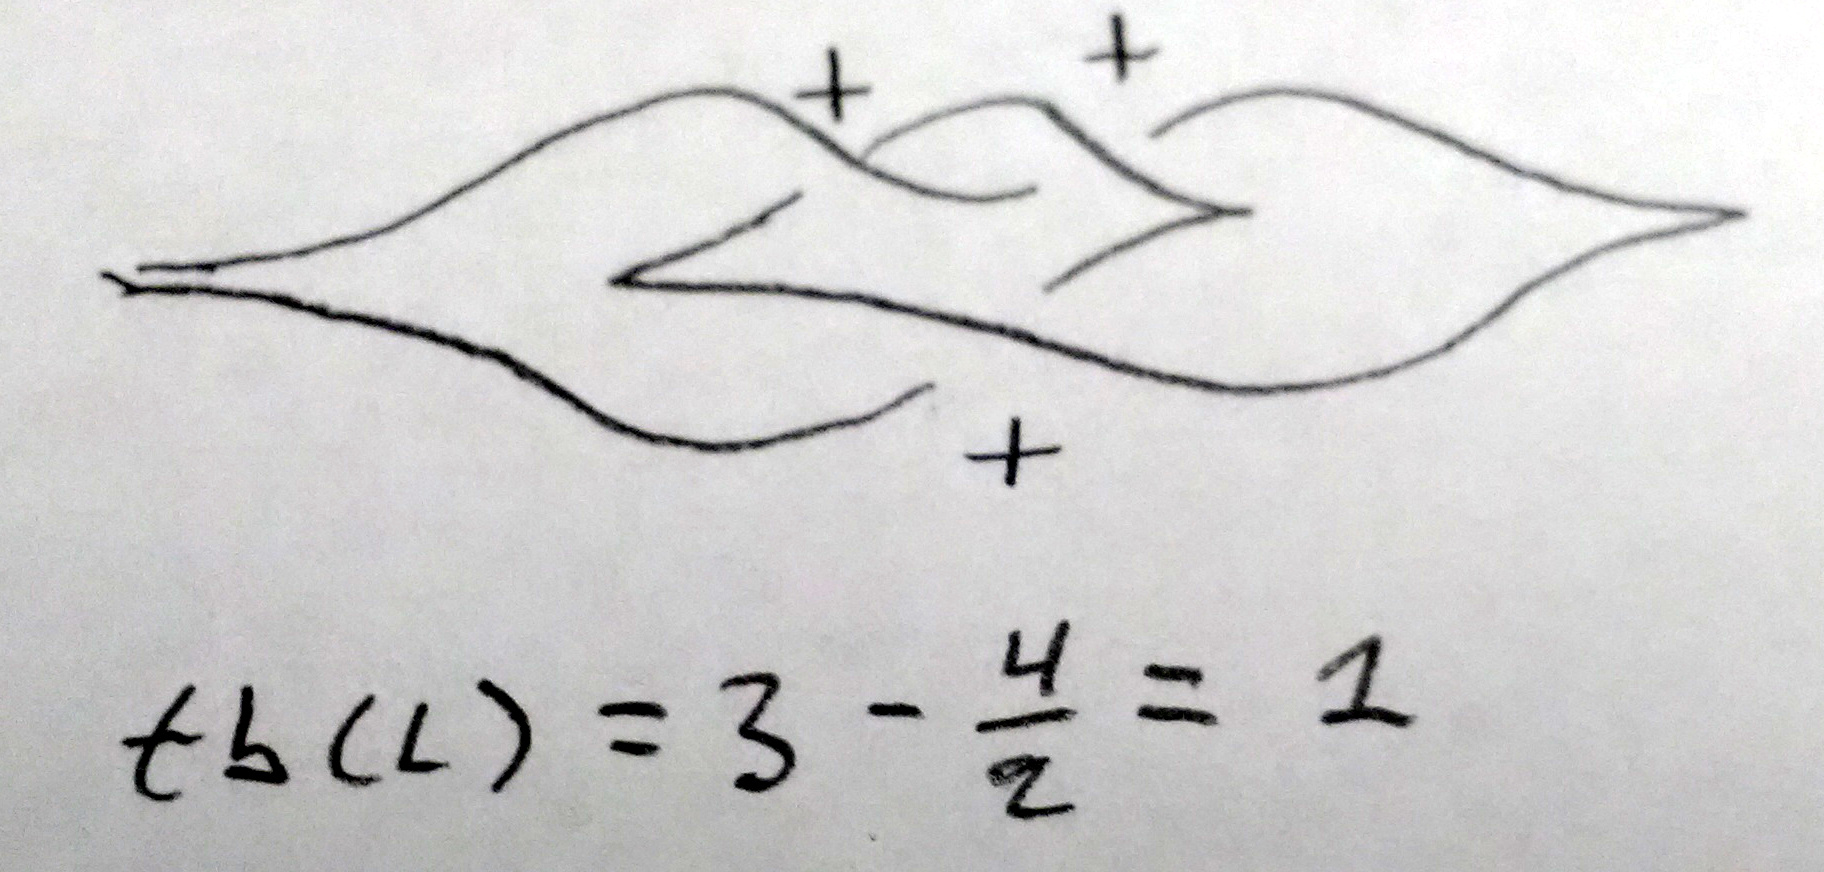
\includegraphics[width=\linewidth]{tbFront.jpg}
    \caption{tb calculation for a front projection of a Legendrian knot}
    \label{fig:knot1}
\end{figure}

Note that the points on the right and left ends that are edge-like and not smooth are
the cusps we are counting. In addition, we have two such points inside the knot
projection, one on each end. This gives us four cusps, and the rest
is easily calculable.


However, given that we have two projections,
is it possible there is a \textit{different} formula for calculating $tb(L)$ using
the \textit{Lagrangian} projection of \textit{L}?

Indeed, there is. For a \textit{Lagrangian} projection of L, all we need is the
\textit{writhe} number for this given knot:

\[tb(L) = writhe(\pi(L)).\]

Let us see a quick example of this:

\begin{figure}[h!]
    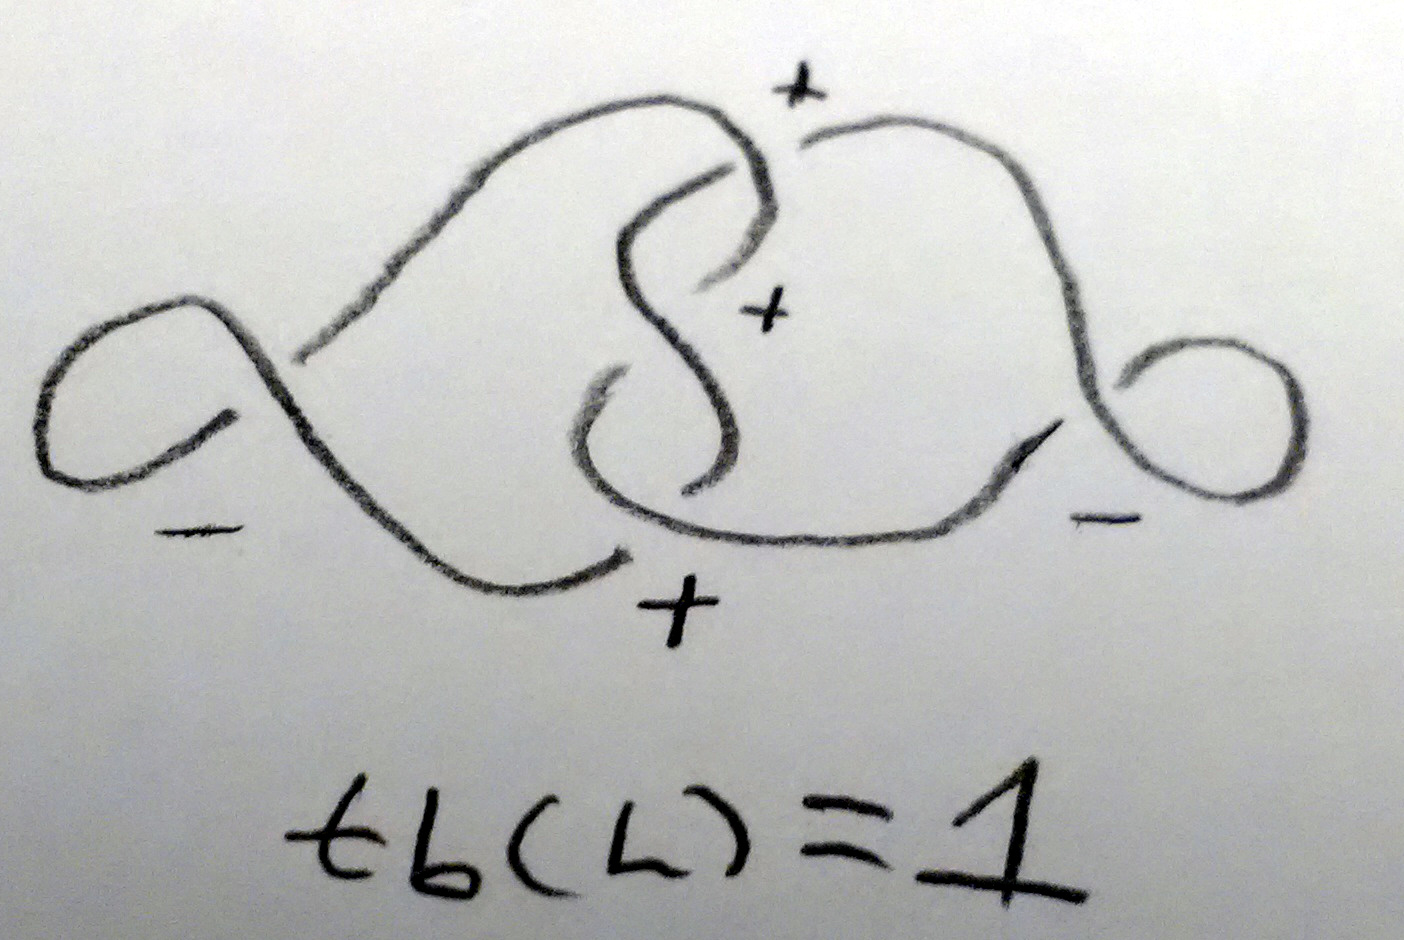
\includegraphics[width=\linewidth]{tbLagr.jpg}
    \caption{tb calculation for a Lagrangian projection of a Legendrian knot.}
    \label{fig:knot1}
\end{figure}


Once again, we note that the actual reasons as to why these formulas work require
upper-level knowledge of geometry and algebra. Those geometric proofs, however,
allow for the simple calculations we see above.

\subsection{Rotation Number}
We take a look at our final classical invariant, the \textit{rotation number}.
Whereas $tb(L)$ focused on the degree to which the contact planes "coiled"/"twisted"
around our knot $L$, \textit{rotation number} is the converse quality: the degree
to which the \textit{knot} twists inside of the contact planes in $\mathbb{R}^3$.

As with $tb(L)$, there are geometric definitions underpinning the formula we will
show. Central to the idea of \textit{rotation number} is the idea of \textit{winding number}:
the amount of times that a curve in a plane goes counterclockwise over some arbitrarily defined
point. We can reason, intuitively, that the degree of twisting a \textit{Legendrian knot} undergoes
around some contact plane is analogous to the \textit{winding number} idea we discussed above.

In any case, what arises from this idea is that we'll need to \textit{orient} our knot projections.
For calculating this number, we'll take a look at the \textit{front} projection.

In order to effectively calculate this number, we'll need the amount of \textit{down} cusps
that the projection has. We note that, if one is orienting the knot projection, then certain
cusps will be oriented \textit{downward} because we travel down them "downwards". We'll denote
these cusps as $D$.

Of course, if there are down cusps, then there are also \textit{up} cusps, cusps that
are oriented \textit{upwards} as a result of the orientation of the knot projection. We will
denote these cusps as \textit{U}.

We have all we need to calculate rotation number, denoted $r(L)$, for
a front projection:

\[r(L) = \frac{1}{2}(D - U).\]

We note that the orientation of the knot can be done in one of two ways,
so this means the numbers for \textit{D} and \textit{U} will be reversed,
potentially changing the sign of \textit{r(L)}. However, the number itself
won't change. To work around this, we note that \textit{r(L)} is really
the \textit{absolute value} of $\frac{1}{2}(D - U).$


With this, we have finished a preliminary discussion of classical invariants.
However, as one will find out if they choose to study \textit{Legendrian knots}
further, these classical invariants will not be enough to distinguish certain
\textit{Legendrian knots} from one another.


% major invariant of the Legendrian knot is the \textit{topological knot type}, here donated as
% $k(L).$ This is a rather intuitive notion.

% The second major invariant is known as the \textit{Thurston-Bennequin invariant}, which essentially
% measures how much coiling a given Legendrian knot has. Legendrian knots have what is called the
% \textit{right cusp number}, essentially a measure of how many local right-cusps there are in its knot diagram.
% These knots also have a quality known as the \textit{writhe } number, which is a measure of
% counting the knot diagram's crossings, but only counting those crossings that have signs. To calculate
% the maximal Thurston-Bennequin number, one can simply subtract the \textit{writhe} - \textit{right cusp number}.

% This number calculated is the invariant. 
% According to the Knot Atlas, the Thurston-Bennequin invariant is not just this number, but rather
% the maximum number of a set of two numbers - the two maximal Thurston-Bennequin numbers
% calculated for both the original knot diagram and its mirror. 

% Rigorously speaking, following in Etnyre's footsteps, we may define the Thurston-Bennequin invariant
% by using the idea of a bundle and its trivialization. Here, we denote a bundle as a \textit{vector bundle},
% a collection of vector spaces that are parameterized by another space. Let us denote a normal, or perpendicular
% bundle of a Legendrian knot $L$ by $v$. A \textit{trivialization} of $v$ is given as identifying $v$ with
% $L \cdot \mathbb{R}^{2}$ (I use \textit{cdot} because I could not find a good symbol for the product).
% Legendrian knots have what are called \textit{line bundles}, which use a Legendrian knot's canonical framing
% to give a framing of $v$ ove $L$.

% Given some normal bundle, we define a number $tw$ as the twisting of $l$ with respect to a
% normal bundle's \textit{preassigned} framing. If $L$ is null-homologous, then $L$ has
% a framing given by a Seifert surface, and the twisting of $L$ with respect to this surface
% is known as the Thurston-Bennequin invariant of $L$, and is denoted as $tb(L).$

% We now come to the last classical invariant: \textit{rotation number}. We define 
% this invariant only for null-homologous knots.
% We assume that $L$ has an embedded, orientable surface. When the contact planes
% for this knot are restricted only to those planes that intersect this surface create
% a trivialization by giving a two-dimensional bundle - as Etnyre states, over a surface with boundary,
% in this case the embedded, orientable surface, any orientable two plane bundle is trivial. Given this
% trivialization, we acquire another trivialization which is the product of $L$ and $\mathbb{R}^{2.}$
% If we denote a non-zero vector field $v$ as one tangent to $L$, pointing in the direction of the orientation given on $L$,
% we can imagine $v$ as a path of vectors in $\mathbb{R}^{2}$, then we realize there is a \textit{winding number} for these vectors,
% and this \textit{winding number} is the rotation number of $L.$ Given that we used the orientation of L in determinng \textit{rotation number},
% we can say the \textit{rotation number} is dependent upon the orientation of $L$ and will accordingly change signs if there is a change in
% orientation.

% We have, in a non-rigorous way, defined our three classical invariants. We now want to find the calculation of the \textit{rotation number}
% as an end to this section.

% We have to simply find how many times a non-zero tangent vector field $v$ that is in $\mathbb{R}^{2}$ goes, or winds, around
% the origin of $\mathbb{R}^{2}$. This involves making a count of how many times our trivialization and $v$ point in the same direction/
% are oriented the same way; this of course creates an intersection between $v$ and our trivialization. We determine the sign
% at each intersection by figuring out if $v$ passes the trivialization clockwise or counter-clockwise ($1, -1$, respectively).
% We then notice that the down and up cusps of our diagram also show whether an intersection will be positive or negative,
% and as this counts the number of times $v$ intersects our trivialization, we just need to divide by two.
% So the formula is:
% \[r(L) = \frac{1}{2}(D - U) \]
% We conclude the rough draft here.
% \section{Chekanov-Eliashberg DGA}

% \textit{This will be added in later, and is not part of the rough draft.}








\begin{thebibliography}{9}
\bibitem{etnyre}
    J. Etnyre,
    \textit{Legendrian and Transversal Knots},
    from: Handbook of Knot Theory,  
    Elsevier B. V.,
    Amsterdam (2005).

\bibitem{sabloffRulings}
    J. Sabloff,
    \textit{Augmentations and Rulings of Legendrian Knots},
    Int. Math. Res. Not. (2005) 1157-1180.

\bibitem{sabloffAMS}
    J. Sabloff,
    \textit{What Is $\ldots$ a Legendrian Knot?},
    AMS Notices, 56 (2009), no. 10, 1282-1284.
\end{thebibliography}

\end{document}
